%%==================================================================%%
%% Author : Tejedo Gonz�lez, Daniel                                 %%
%%          S�nchez Barreiro, Pablo                                 %%
%% Version: 1.0, 27/11/2012                                         %%                   %%                                                                  %%
%% Memoria del Proyecto Fin de Carrera                              %%
%% Gram�tica,  archivo raiz                                       %%
%%==================================================================%%

\chapterheader{Creaci�n de la gram�tica}{Creaci�n de la gram�tica}
\label{chap:gramatica}

Una vez definida la sintaxis abstracta de nuestro lenguaje, el siguiente paso era definir la sintaxis concreta de nuestro lenguaje, que en nuestro caso ser�a una sintaxis textual. Para ello hicimos uso de la herramienta EMFText. Este cap�tulo describe el proceso de desarrollo de dicha sintaxis textual concreta de acuerdo al proceso impuesto por EMFText.

\chaptertoc

%%=================================================================%%
%% NOTA(Pablo) : Lo mismo que con el cap�tulo 3, escribe una       %% 
%%               peque�a introducci�n al cap�tulo                  %%
%%=================================================================%%

\section{Introducci�n}
\label{sec:gram:introduccion}
%%==================================================================%%
%% Author : Tejedo Gonz�lez, Daniel                                 %%
%%          S�nchez Barreiro, Pablo                                 %%
%% Version: 1.0, 27/11/2012                                         %%                   
%% Version: 2.0, 09/02/2013                                         %%                   
%%                                                                  %%
%% Memoria del Proyecto Fin de Carrera                              %%
%% Gram�tica, Introducci�n                                                %%
%%==================================================================%%

Siguiendo la metodolog�a impuesta por la Ingenier�a de Lenguajes Dirigida por Modelos, la siguiente parte del desarrollo de nuestro lenguaje pasa por definir la sintaxis concreta textual del mismo. Para poder llevar a cabo esta tarea es necesario escribir una gram�tica, que se encargar� de transformar el c�digo que escribamos en nuestro lenguaje en instancias v�lidas del metamodelo inicial. La captura de requisitos de la gram�tica es pr�cticamente id�ntica a la que se hizo en el cap�tulo anterior para dise�ar el metamodelo, pues en ambos casos es necesario conocer las operaciones del lenguaje y su sintaxis. 

El cap�tulo se estrucurar� del siguiente modo: en primer lugar hablaremos sin entrar en mucho detalle de la herramienta \emph{EMFText}, que es la que hemos escogido para dise�ar nuestra gram�tica. A continuaci�n, y en la misma secci�n, describiremos esta gram�tica y las partes que la componen. Por �ltimo mostraremos las pruebas a las que fue sometida para corroborar que su funcionamiento era el apropiado.

%%=================================================================%%
%% NOTA(Pablo): Los requisitos de la gram�tica quedan 
%%              pr�cticamente definidos en el art�culo que te 
%%              mand�, y que est� descrita en el cap�tulo 
%%              anterior, por tanto no hace falta enrrollarse. 
%%              Se puede fusionar con la secci�n de introducci�n
%%=================================================================%%
%%
%% \section{Captura de requisitos}
%% \label{sec:gram:requisitos}
%% %%==================================================================%%
%% Author : Tejedo Gonz�lez, Daniel                                 %%
%%          S�nchez Barreiro, Pablo                                 %%
%% Version: 1.0, 25/11/2012                                         %%
%% Version: 2.0, 06/02/2013                                         %%
%%                                                                  %%
%% Memoria del Proyecto Fin de Carrera                              %%
%% Sintaxis abstracta, requisitos                                   %%
%%==================================================================%%

El primer paso para desarrollar nuestro lenguaje era conocer qu� aspecto deb�a tener nuestro lenguaje y qu� restricciones deb�a satisfacer. Es decir, en primer lugar debemos realizar un proceso que podemos denominar de captura de requisitos para poder comprender qu� es lo que tiene que hacer exactamente el lenguaje que se pretende crear.

Concretamente nuestro lenguaje hab�a sido pr�cticamente definido por el profesor Pablo S�nchez, del Departamento de Matem�ticas, Estad�stica y Computaci�n de la Universidad de Cantabria, mediante notaci�n BNF. Dicha gram�tica, se muestra en la Figura~\ref{fig:constraintBNF}. Las ideas subyacentes a dicho lenguaje son las que se describen a continuaci�n. 

\begin{figure}[!tb]
    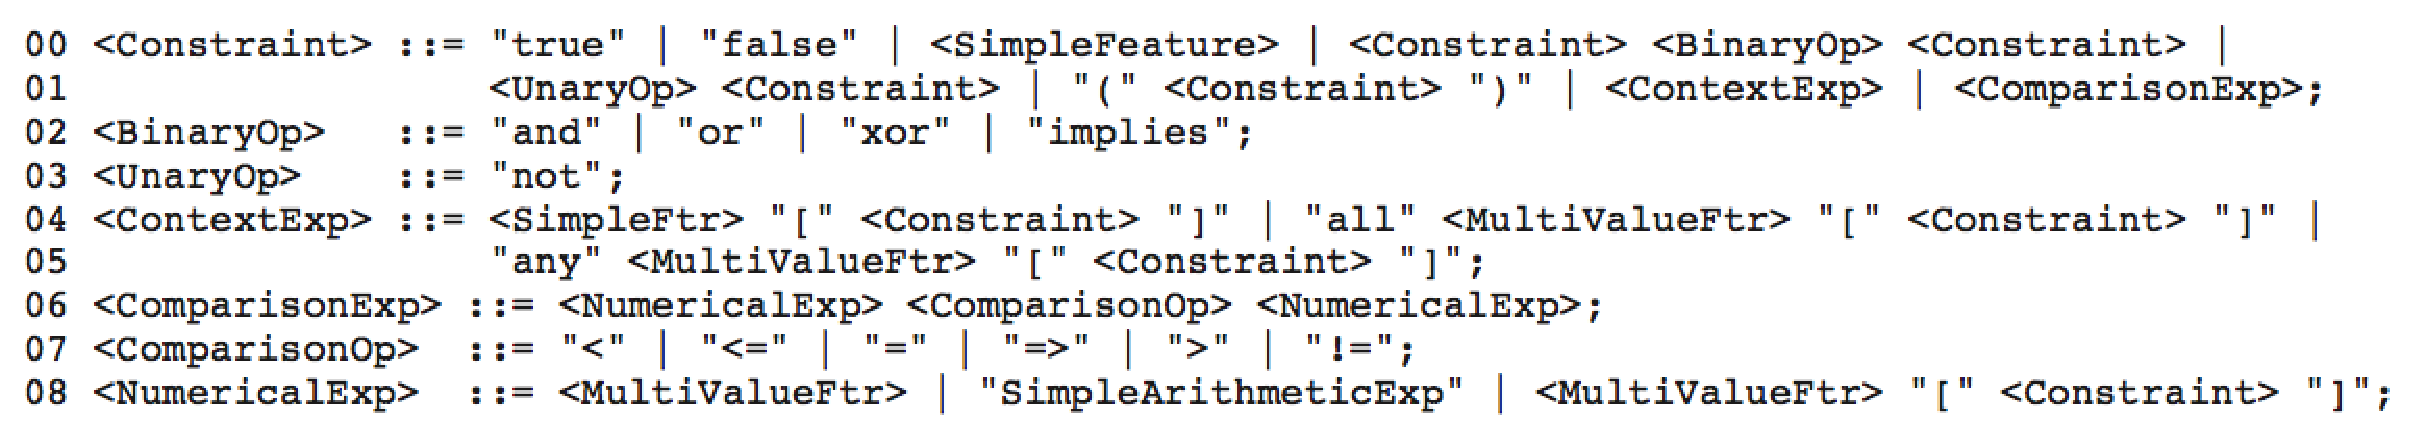
\includegraphics[scale=0.3]{metamodelo/constraintBNF.eps}
    \caption{Gram�tica en notaci�n BNF del lenguaje HCL}
    \label{fig:constraintBNF}
\end{figure}

En dicho lenguaje, una \emph{restricci�n} es una expresi�n l�gica que se puede evaluar a verdadero o falso. Una restricci�n puede ser simplemente un literal, es decir, $true$ o $false$, que se evaluar� a verdadero y falso respectivamente. Una restricci�n tambi�n puede ser una caracter�stica simple, es decir, una caracter�stica que puede aparecer en las configuraciones como m�ximo una vez. Una caracter�stica simple se eval�a a verdadero si ha sido seleccionada, y a falso en caso contrario.

Las caracter�sticas clonables son aquellas que pueden ser seleccionadas m�s de una vez en las configuraciones que construyamos sobre nuestro �rbol de caracter�sticas. Una caracter�stica clonable se eval�an como un n�mero entero positivo, incluido el cero. Ese n�mero representa el n�mero de clones que la caracter�stica posee dentro de una configuraci�n, o dicho de otro modo, el n�mero de veces que ha sido seleccionada. El hecho de que se eval�en como si fueran n�meros permite la inclusi�n de operaciones de comparaci�n entre distintas caracter�sticas clonables. Las operaciones de comparaci�n que se han de implementar son las siguientes: $<$,$<$=,$>$,$>=$,$=$,$!=$. Adem�s, tambi�n se puede utilizar el valor de las caracter�sticas clonables para implementar operaciones aritm�ticas b�sicas, tales como la suma, la resta, la multiplicaci�n y la divisi�n. Estas expresiones a su vez se pueden utilizar como subexpresiones, u operandos, dentro de las operaciones de comparaci�n. Las expresiones de comparaci�n se eval�an a verdadero o falso, y tambi�n pueden ser usadas como subexpresiones para crear expresiones l�gicas m�s complejas.

%%============================================================================%%
%% NOTA(Pablo) : Poner un ejemplo de este tipo de restricciones y explicarlas %%
%%============================================================================%%

Tal y como muestra la Figura~\ref{fig:constraintBNF}, una restricci�n tambi�n puede especificar un contexto concreto en el que poder evaluarla. Esto puede hacerse de varias maneras. Se puede especificar un contexto para una restricci�n poni�ndola entre corchetes y especificando el nombre de una caracter�stica al principio de la expresi�n. La caracter�stica usada como contexto puede ser tanto simple como m�ltiple. En el primer caso, la restricci�n s�lo ser� evaluada en el sub�rbol de la configuraci�n cuya ra�z sea la caracter�stica especificada.

%%============================================================================%%
%% NOTA(Pablo) : Poner un ejemplo y explicarlo                                %%
%%============================================================================%%

En el segundo caso entran en juego los operadores $all$ (para todo) y $any$ (existe). La operaci�n $all$ solo se evaluar� a verdadero si la restricci�n entre corchetes se cumple para todas las instancias de la caracter�stica clonable que act�a como contexto. En caso contrario, la operaci�n se evaluar� a falso. La operaci�n $any$ se evaluar� a verdadero si la restricci�n entre corchetes se cumple al menos una vez para todas las instancia de la caracter�stica clonable que act�a como contexto. Si la restricci�n no se cumple para ninguna de las selecciones, la operaci�n $any$ se evaluar� a falso.

%%============================================================================%%
%% NOTA(Pablo) : Poner un ejemplo y explicarlo                                %%
%%============================================================================%%

Merece la pena se�alar que una caracter�stica puede ser considera simple en un contexto determinado y clonable o m�ltiple en otro. Por ejemplo, la caracter�stica $LightMng$ es clonable en el contexto de $RoomFacilities$, pero simple en el contexto de $GeneralFacilities$. Debido a eso la caracter�stica $LightMng$ no puede ser utilizada sin especificar el contexto en el que est� ubicada, pues podr�a provocar un resultado no esperado o err�neo.

En la restricci�n $any Room[RoomFacilities[LightMng]]$ se pueden apreciar los dos diferentes usos para la operaci�n de contexto. Los corchetes externos indican a la operaci�n any que hay que aplicar la restricci�n a todas las habitaciones. Los corchetes internos indican que la caracter�stica $LightMng$ a la que se est� haciendo referencia es la hija de $RoomFacilities$ y no cualquier otra.

Adem�s nuestro lenguaje deb�a permitir vincular un modelo de caracter�sticas sobre el cual se definir�n un conjunto de restricciones externas. Este modelo se utilizar�, por ejemplo, para comprobar que los s�mbolos que aparecen como nombres de caracter�sticas en las restricciones se refieren a caracter�sticas que realmente existen en el �rbol de caracter�sticas. Por ejemplo, una restricci�n del tipo $AdvancedHeating => Heating$ carecer�a de sentido si algunas de las caracter�sticas $AdvancedHeating$ o $Heating$ no apareciesen en el �rbol de caracter�sticas sobre el cual estamos definiendo restricciones.

%%======================================================================================%%
%% NOTA(Pablo): Esto posiblemente sobre al introducir la traducci�n de la Secci�n III.
%%              Si es as�, eliminarla.
%%              Si los conceptos de restricci�n con contexto y operaci�n cuantificada
%%              no apareciesen, meter esta clasificaci�n pero resumida
%%======================================================================================%%
%%
%% De entre todos esos requisitos b�sicos, es necesario entrar en detalle en el n�mero 3
%% y enumerar la lista de operaciones que pueden ser definidas por nuestro lenguaje. Se
%% pueden clasificar en los siguientes tipos: \\
%%
%% - L�gicas: Son operaciones cuyos operandos han de ser caracter�sticas sin
%%   cardinalidad (tambi�n llamadas caracter�sticas simples), y que se evaluan a
%%   verdadero o falso. Entre las operaciones l�gicas encontramos las cl�sicas not,
%%   and, or, xor e implica.
%%
%% - Num�ricas: Sus operandos han de ser caracter�sticas con cardinalidad (tambi�n
%%   llamadas caracter�sticas m�ltiples) o simplemente n�meros. Su resultado se evalua
%%   con un valor num�rico. Las operaciones num�ricas a implementar son la suma, resta,
%%   multiplicaci�n y divisi�n.
%%
%% - Comparativas: Sus operandos han de ser caracter�sticas m�ltiples o simplemente n�meros,
%%   pero su resultado se evalua con un valor booleano. Las operaciones de comparaci�n a
%%   implementar son igual que, mayor que, menor que, distinto que, mayor o igual que y menor
%%   o igual que.
%%
%% - Operaci�n de contexto: Operaci�n que permite hacer referencia a una caracter�stica
%%   hija de otra caracter�stica. Esta operaci�n tiene sentido para seleccionar
%%   caracter�sticas cuyo nombre pueda estar repetido pero que tengan contextos diferentes.
%%   Por ejemplo, en el modelo de caracter�sticas SmartHome de la figura \ref{figsmarthome}
%%   podemos observar que la caracter�stica HeaterMng est� presente en muchos contextos
%%   diferentes. Esta operaci�n es necesaria para poder saber con seguridad a cual de esos
%%   contextos estamos aplicando la restricci�n.
%%
%% - Operaci�n de selecci�n: Operaci�n que corresponde a los operadores l�gicos cl�sicos
%%   "para todo" o "existe", y que tiene la misma funcionalidad. Evalua si una restricci�n
%%   se cumple para todos los casos en que puede existir  o si se cumple en alguno de los
%%   casos. Por ejemplo, en el modelo de la figura \ref{figsmarthome} se podr�a evaluar una
%%   restricci�n para cada una de las habitaciones que hayan sido definidas, y saber si se
%%  cumple en todas, en alguna o en ninguna.
%%
%%======================================================================================%%

Utilizando esta informaci�n como base, procedimos a crear el correspondiente metamodelo en Ecore para nuestro lenguaje.



%%
%%=================================================================%%

\section{Implementaci�n de la Gram�tica}
\label{sec:gram:design}
%%==================================================================%%
%% Author : Tejedo Gonz�lez, Daniel                                 %%
%%          S�nchez Barreiro, Pablo                                 %%
%% Version: 1.0, 27/11/2012                                         %%                   
%% Version: 2.0, 09/02/2013                                         %%                   
%%                                                                  %%
%% Memoria del Proyecto Fin de Carrera                              %%
%% Gram�tica, Dise�o                                                %%
%%==================================================================%%

Una vez han sido definidas las caracter�sticas que queremos que nuestra sintaxis textual posea, el siguiente paso es dise�ar una gram�tica que se ajuste a ellas. EMFText es la herramienta que utilizaremos para implementar esta gram�tica. 

El dise�o de la gram�tica pasa por asignar una serie de reglas a las metaclases, de modo que EMFText sea capaz de reconocer esas reglas en las expresiones de nuestro lenguaje y asociarlas a la metaclase correspondiente. En cuanto la reconozca, a�adir� una instancia de la misma, con los atributos correspondientes debidamente inicializados, a la instancia global del metamodelo.

Adem�s de las reglas, en EMFText hay que definir otra serie de cla�sulas que permiten configurar ciertos aspectos de la gram�tica. Para explicar tanto estas directrices como las reglas de las metaclases nos apoyaremos en la gram�tica dise�ada, y explicaremos l�nea a l�nea el significado de las instrucciones que la componen. La Figura~\ref{fig:initGram} muestra las primeras 23 l�neas de la gram�tica para nuestro lenguaje. 
%%=================================================================%%
%% NOTA(Pablo): Refresca aqu� un poco el proceso de desarrollo de  %%
%%              gram�ticas con EMFText, en uno o dos parr�fos a    %%
%%              muy alto nivel                                     %%   
%%=================================================================%%

%%=================================================================%%
%% NOTA(Pablo): Tal como est� escrito, es dif�cil seguir el hilo   %%
%%              argumental, vuelvo a escribirlo de forma top-down, %%
%%              describiendo, sin enrollarte mucho, lo que aparece %%
%%              en las figuras. Empieza por la segunda, por la     %%
%%              l�nea 1, y sigue para abajo                        %%
%%              Piensa en a�adirle n�meros de l�neas a las figuras %%
%%              para hacer m�s f�cil su descripci�n.               %%
%%              Haz especial hincapi� en como se relacionan la     %% 
%%              gram�tica con el metamodelo. 
%%              Evista el t�rmino producci�n, que es muy 
%%              espec�fico de procesdores de lenguajes, y no todos
%%              los miembros del tribunal lo van a entender
%%              Planteate usar el entorno listing para mostrar 
%%              c�digo
%%=================================================================%%

%%=================================================================%%
%% NOTA(Pablo): Estas figuras se ven fatal, no las metas como      %%
%%              capturas de pantalla o p�salas a EPS mejor         %%
%%=================================================================%%

\begin{figure}[t]
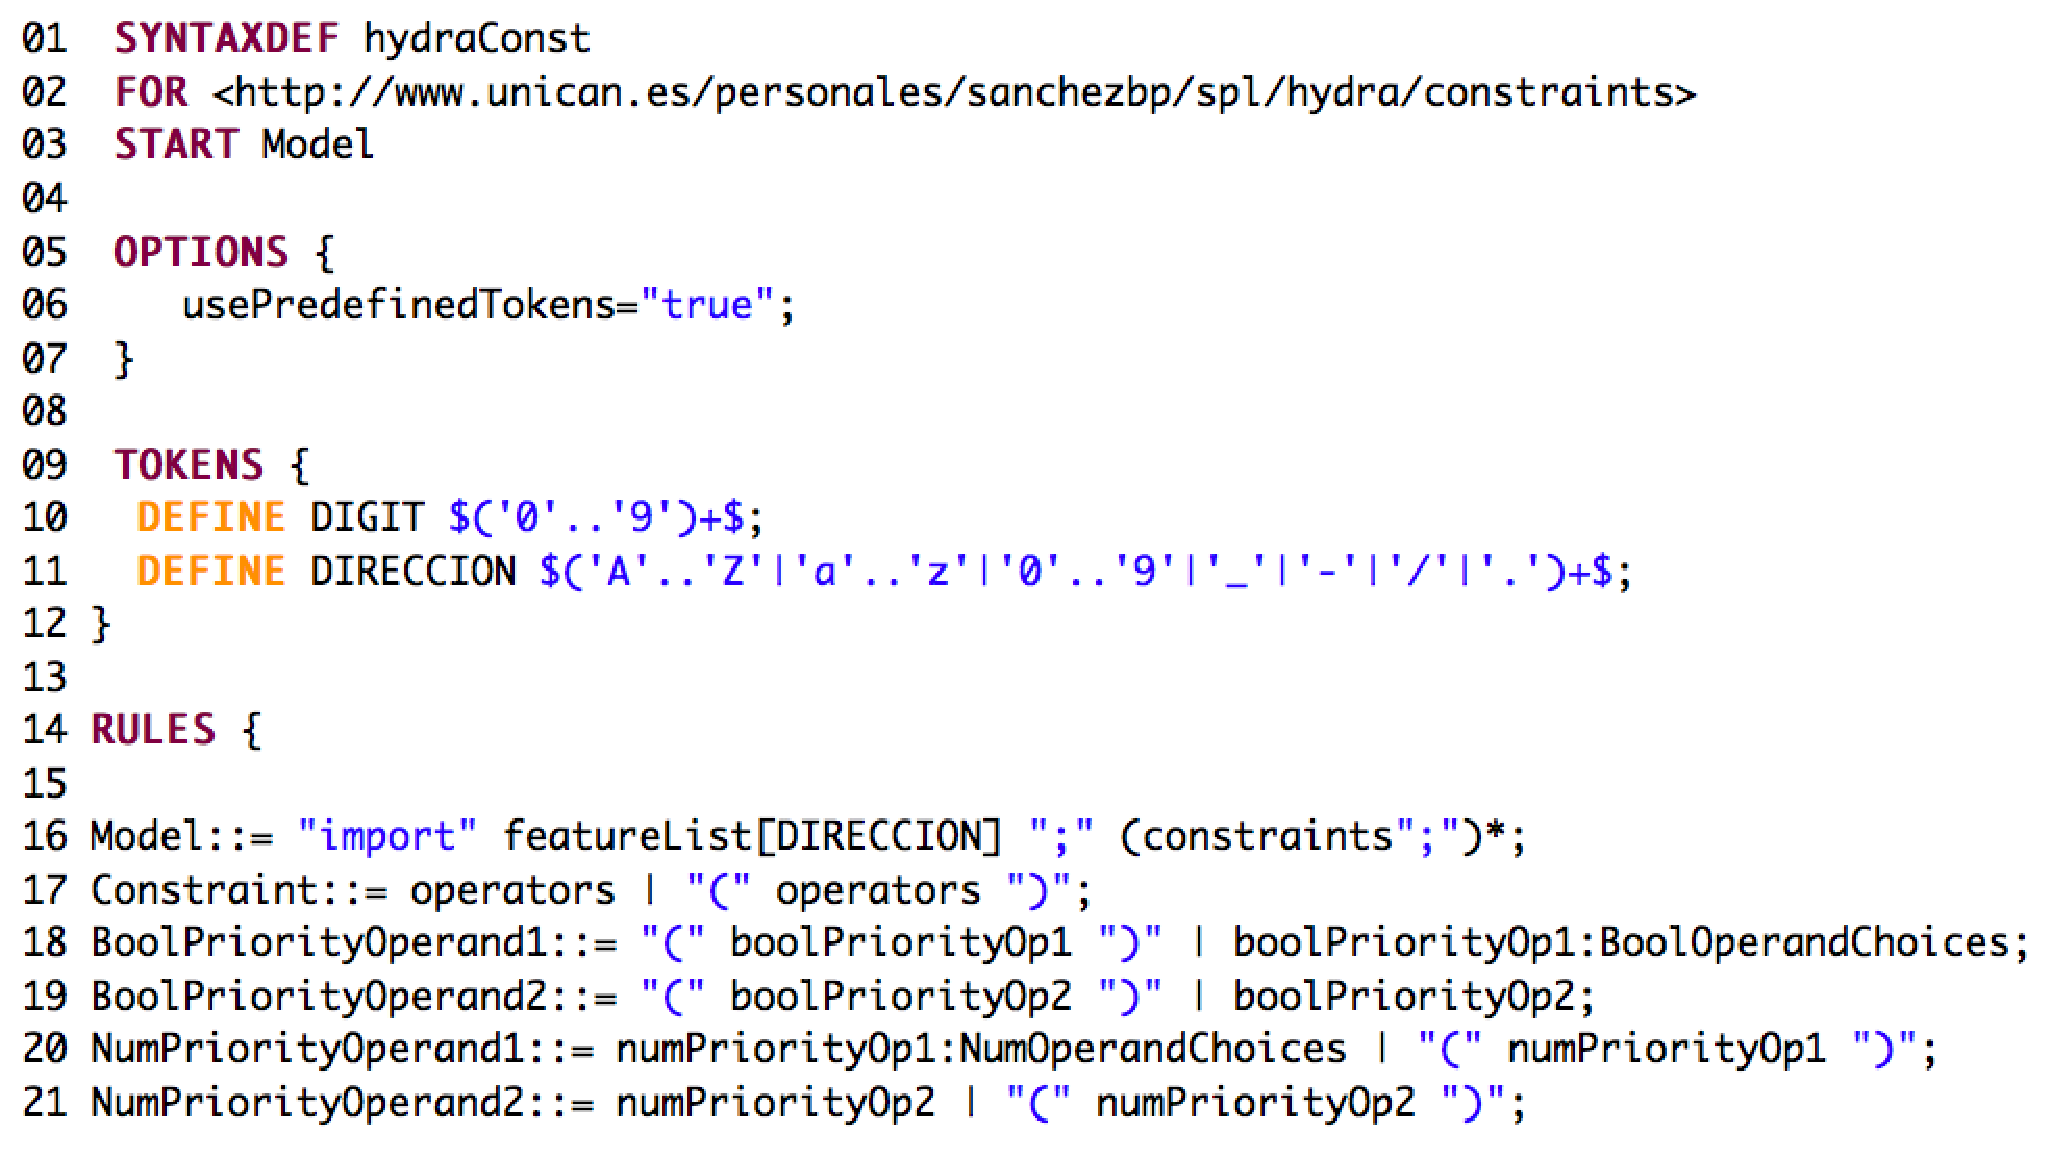
\includegraphics[scale=0.35]{gramatica/iniciogram.eps}
\caption{Implementaci�n del inicio de la gram�tica con EMFText. Con las figuras \ref{fig:opersUno} y \ref{fig:opersDos} se completa la gram�tica}
\label{fig:initGram}
\end{figure}

La primera l�nea muestra la cla�sula SYNTAXDEF, que sirve para indicar la extensi�n que queramos que tengan los ficheros correspondientes a nuestro lenguaje. En nuestro caso, hemos elegido la extensi�n \emph{hydraconst}. A continuaci�n, la directriz FOR sirve para vincular la gram�tica con el metamodelo mediante una direcci�n de Eclipse llamada \emph{URI}. La siguiente l�nea contiene la cl�usula START, que indica cu�l es la metaclase inicial del metamodelo, es decir, la primera a la que se le aplica una regla. Cualqueir gram�tica que se quiera construir en EMFText ha de empezar por estas tres directrices.

Las l�neas de [05-07] corresponden al bloque OPTIONS. Dentro de este bloque EMFText permite especificar diversas opciones para configurar nuestra gram�tica de diversos modos, que en su mayor�a afectan a la posterior generaci�n del c�digo que implementar�  el lenguaje. En nuestro caso solo hemos activado una opci�n, que permite usar los Tokens definidos por defecto en EMFText.

Entre las l�neas [09-12] se encuentra el bloque TOKENS. Este bloque sirve para definir los Tokens que usaremos en nuestra gram�tica. Un Token es un elemento terminal, es decir, uno cuyo derivaci�n no supone ninguna regla adicional para la gram�tica. En nuestro caso usaremos los Tokens para inicializar diversos atributos del metamodelo. El Token DIGIT ser� el que d� valor al atributo \emph{numValue} de la metaclase \emph{Number}, y el token DIRECCION ser� el utilizado para inicializar el atributo \emph{featureList} de la metaclase Model. Adem�s, usaremos el token TEXT para inicializar el atributo \emph{featureName} de las metaclases \emph{SimpleFeature} y \emph{MultipleFeature}. Este Token no hay que definirlo, ya que est� disponible por defecto al habilitar la opci�n previa \emph{usePredefinedTokens}.

Desde la l�nea 14 y hasta el final de la gram�tica estar� contenido el bloque RULES, que es en el que se definen las reglas de las que habl�bamos. La l�nea 16 contiene la regla de la metaclase inicial, Model. Esto significa que los textos que escribamos en nuestros lenguajes han de empezar siguiendo esta regla. En ella se define que la primera l�nea de cualquier c�digo escrito en nuestro lenguaje ha de empezar por la palabra reservada \emph{import}, y a continuaci�n se introduce la direcci�n que contiene el modelo de caracter�sticas sobre el que queremos aplicar las restricciones. Esta direcci�n se define por el Token DIRECCION y se guarda en el atributo \emph{featureList}. A partir de ah�, se indica que se han de escribir las restricciones.

La l�nea 17 contiene la regla correspondiente a la metaclase \emph{Constraint}. En ella simplemente se indica que a continuaci�n hay que escribir los diversos operadores, y se actualizan en el metamodelo las relaci�n llamada \emph{operators}. Las l�neas [18-21] sirven para implementar la prioridad en las operaciones, es decir, permitir la inclusi�n de par�ntesis en las operaciones.

\begin{figure}[t]
    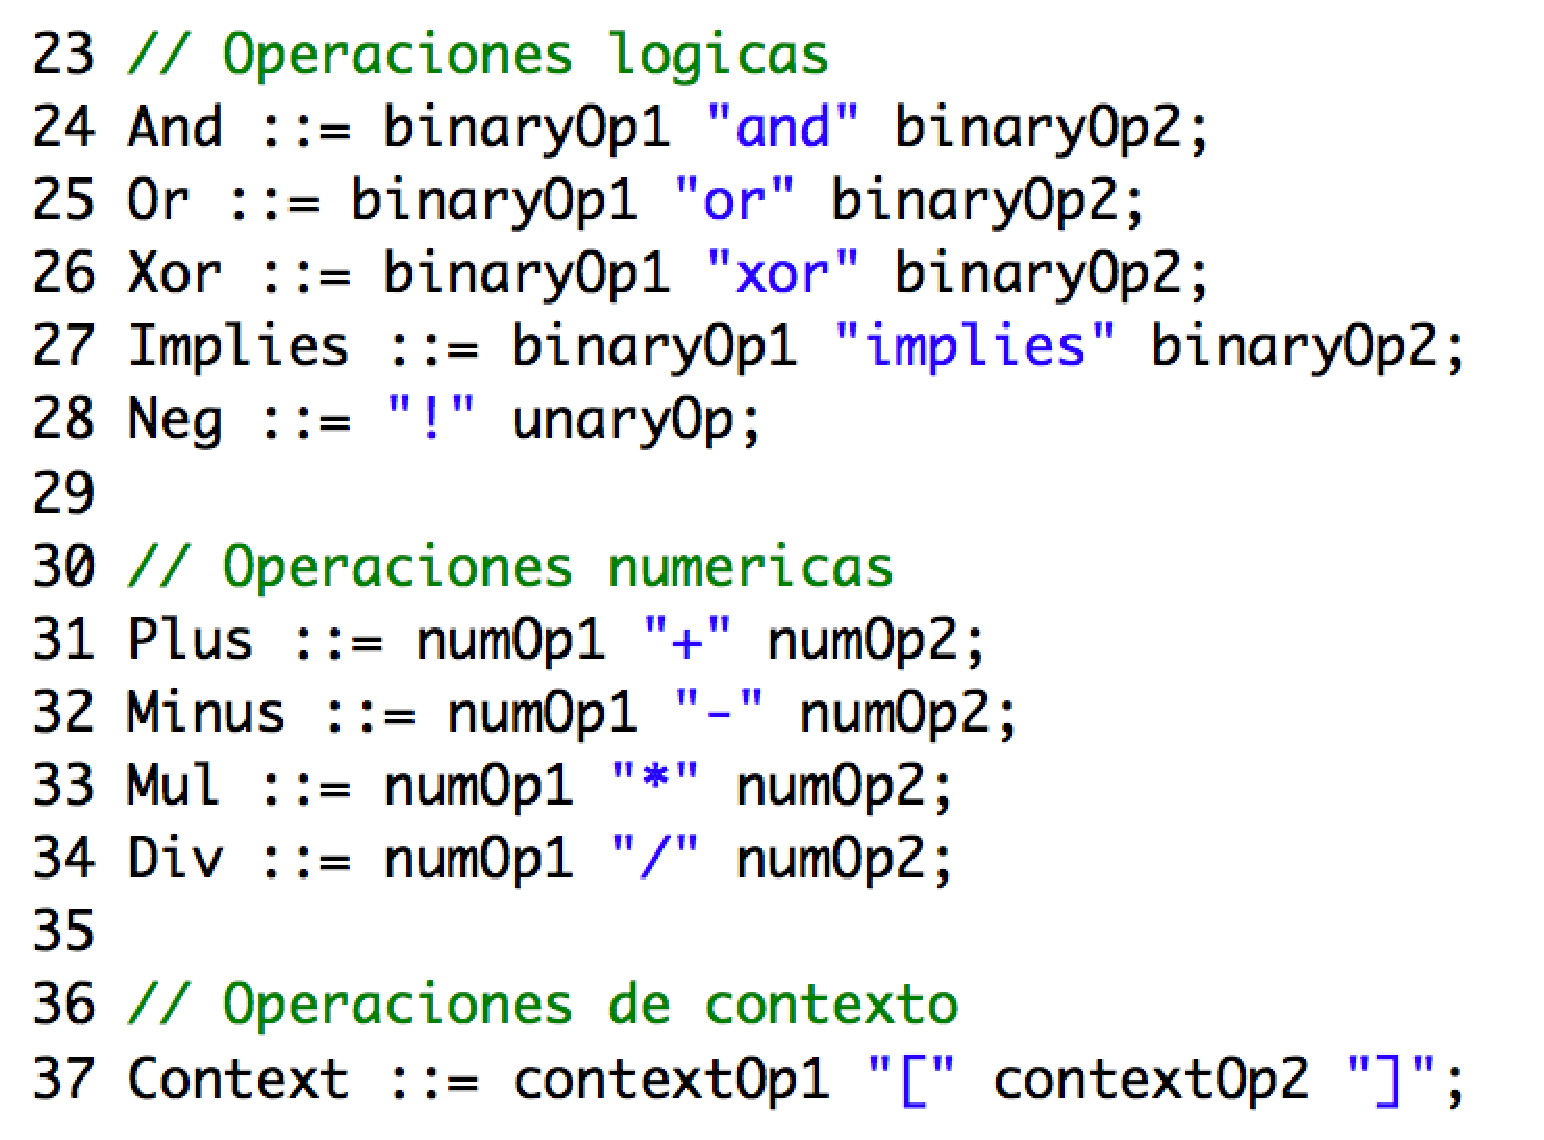
\includegraphics[scale=0.3]{gramatica/operaciones1.eps}
    \caption{Primera parte de la implementaci�n de las operaciones de nuestro editor com EMFText}
    \label{fig:opersUno}
\end{figure}

La Figura~\ref{fig:opersUno} contin�a directamente el trozo de gram�tica de la Figura~\ref{fig:initGram} y muestra las reglas correspondientes a una parte de las operaciones. 

Las l�neas [23-28] muestran las reglas para las operaciones l�gicas. Indican que la palabra reservada para la operaci�n de la metaclase \emph{And} es \emph{and}, y del mismo modo con las metaclases \emph{Or}, \emph{Xor} e \emph{Implies}. La palabra reservada para la operaci�n de la metaclase \emph{Not} es !. En estas reglas tambi�n se inicializan las relaciones \emph{binaryOp1}, \emph{binaryOp2} y \emph{unaryOp} al valor correspondiente. 

Las l�neas [30-34] muestran las reglas para las operaciones aritm�ticas. Indican que la palabra reservada para la operaci�n de la metaclase \emph{Plus} es $+$, para \emph{Minus} es $-$, para \emph{Mul} es $*$ y para \emph{Div} es $/$. En estas reglas tambi�n se inicializan las relaciones \emph{numOp1} y \emph{numOp2} al valor correspondiente. 

La l�nea 37 implementa la regla para la operaci�n correspondiente a la metaclase \emph{Context}. En ella se indica que un contexto se compone del operador \emph{contextOp2} rodeado entre corchetes precedido del operador \emph{contextOp1}. Ambos operadores son instanciados en sus debidas relaciones en el metamodelo.

\begin{figure}[t]
    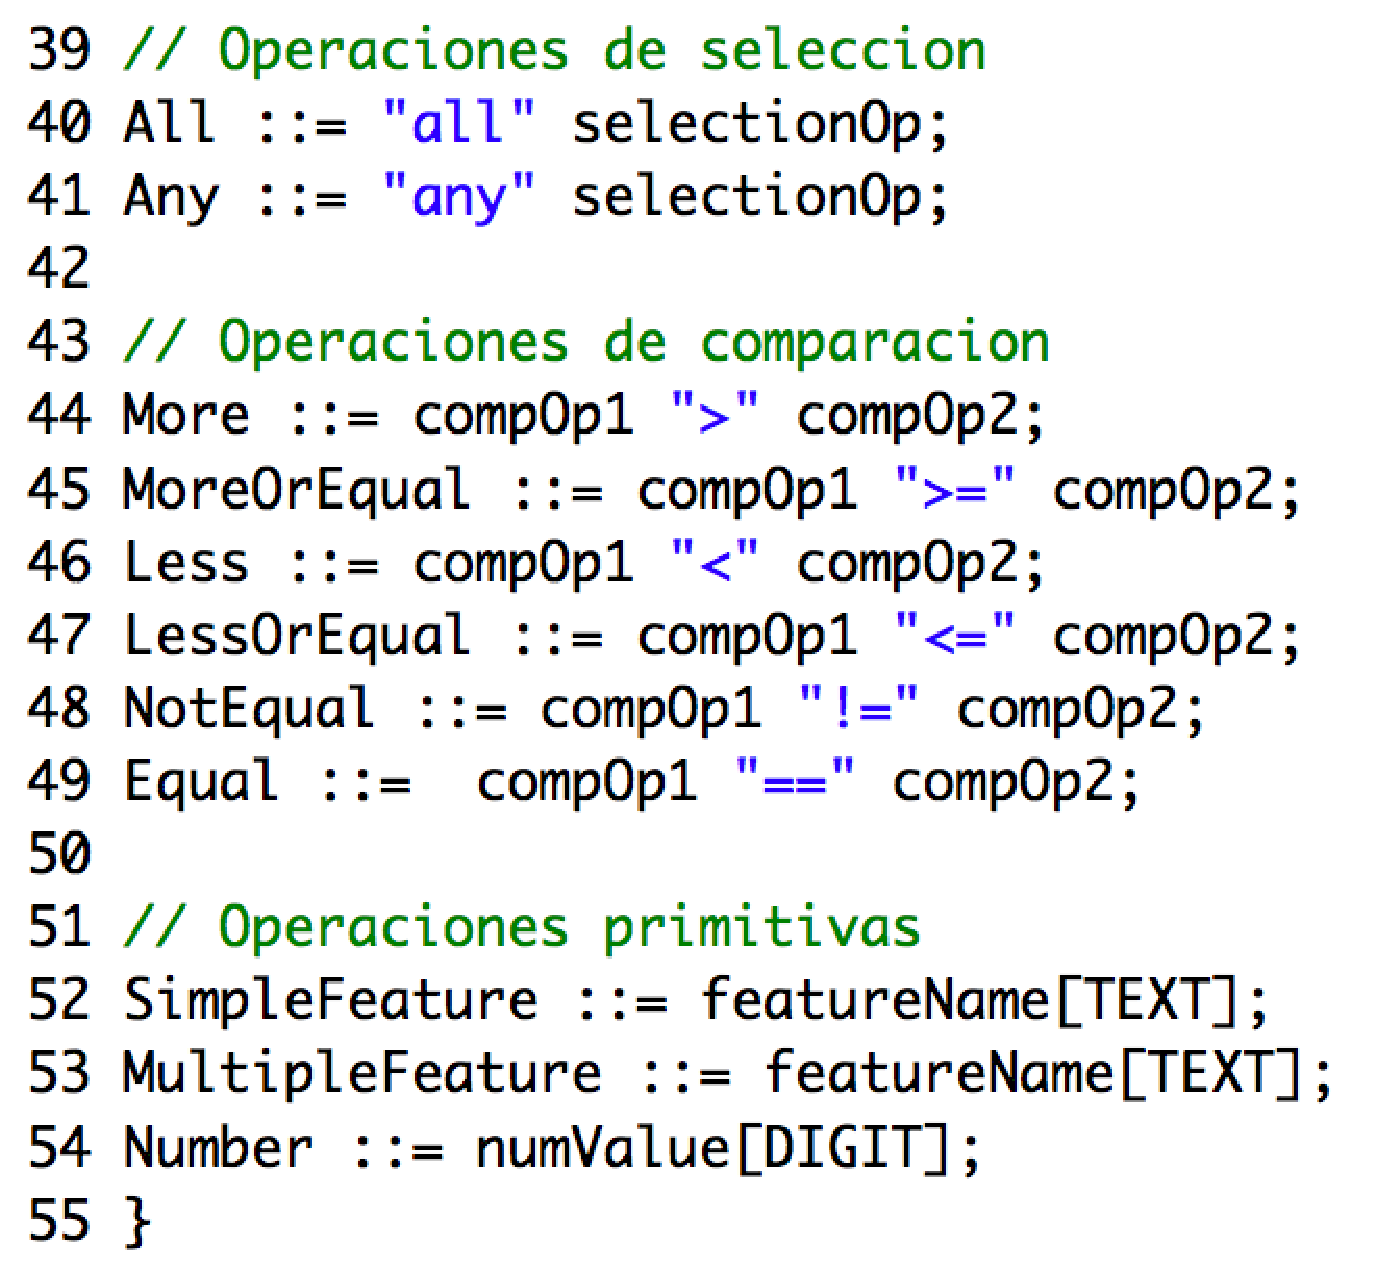
\includegraphics[scale=0.3]{gramatica/operaciones2.eps}
    \caption{Segunda parte de la implementaci�n de las operaciones de nuestro editor com EMFText}
    \label{fig:opersDos}
\end{figure}

La Figura~\ref{fig:opersDos} contin�a directamente el trozo de gram�tica de la Figura~\ref{fig:opersUno} y muestra la siguiente parte de la implementaci�n de las reglas de las operaciones.

Las l�neas [39-40] muestran las reglas para las operaciones correspondientes a las metaclases \emph{All} y \emph{Any}. En ambas se indica que la palabra reservada que las identifica es \emph{all} y \emph{any} respectivamente, y que a continuaci�n se ha de indicar el operador \emph{selectionOp}. Si miramos el metamodelo, veremos que este operador corresponde a una relaci�n con una operaci�n de contexto, con lo cual en este momento habr�a que introducir una restricci�n entre corchetes precedida de una caracter�stica que marque el contexto en que se eval�a. 

Las l�neas [43-49] muestran las reglas para las operaciones de comparaci�n. Indican que la palabra reservada para la operaci�n de la metaclase \emph{More} es $>$, para \emph{MoreOrEqual} es $>=$, para \emph{Less} es $<$, para \emph{LessOrEqual} es $<=$, para \emph{NotEqual} es $!=$ y para \emph{Equal} es $==$. En estas reglas tambi�n se inicializan las relaciones \emph{compOp1} y \emph{compOp2} al valor correspondiente. 

Para finalizar, las l�neas [51-54] muestran las operaciones primitivas. En el lenguaje, estas reglas corresponden a inicializar el atributo \emph{featureName} con el nombre de la caracter�stica que hayamos introducido, y del mismo modo, el atributo \emph{numValue} con el del n�mero que hayamos escrito.
%La parte m�s trivial e inmediata del dise�o de la gram�tica es la concerniente a la implementaci�n de las operaciones, pues las producciones necesarias simplemente requieren la inclusi�n de los operandos involucrados y los caracteres que deseemos que definan la operaci�n. La figura \ref{figopers} muestra la implementaci�n de estas operaciones.
%
%\begin{figure}[t]
%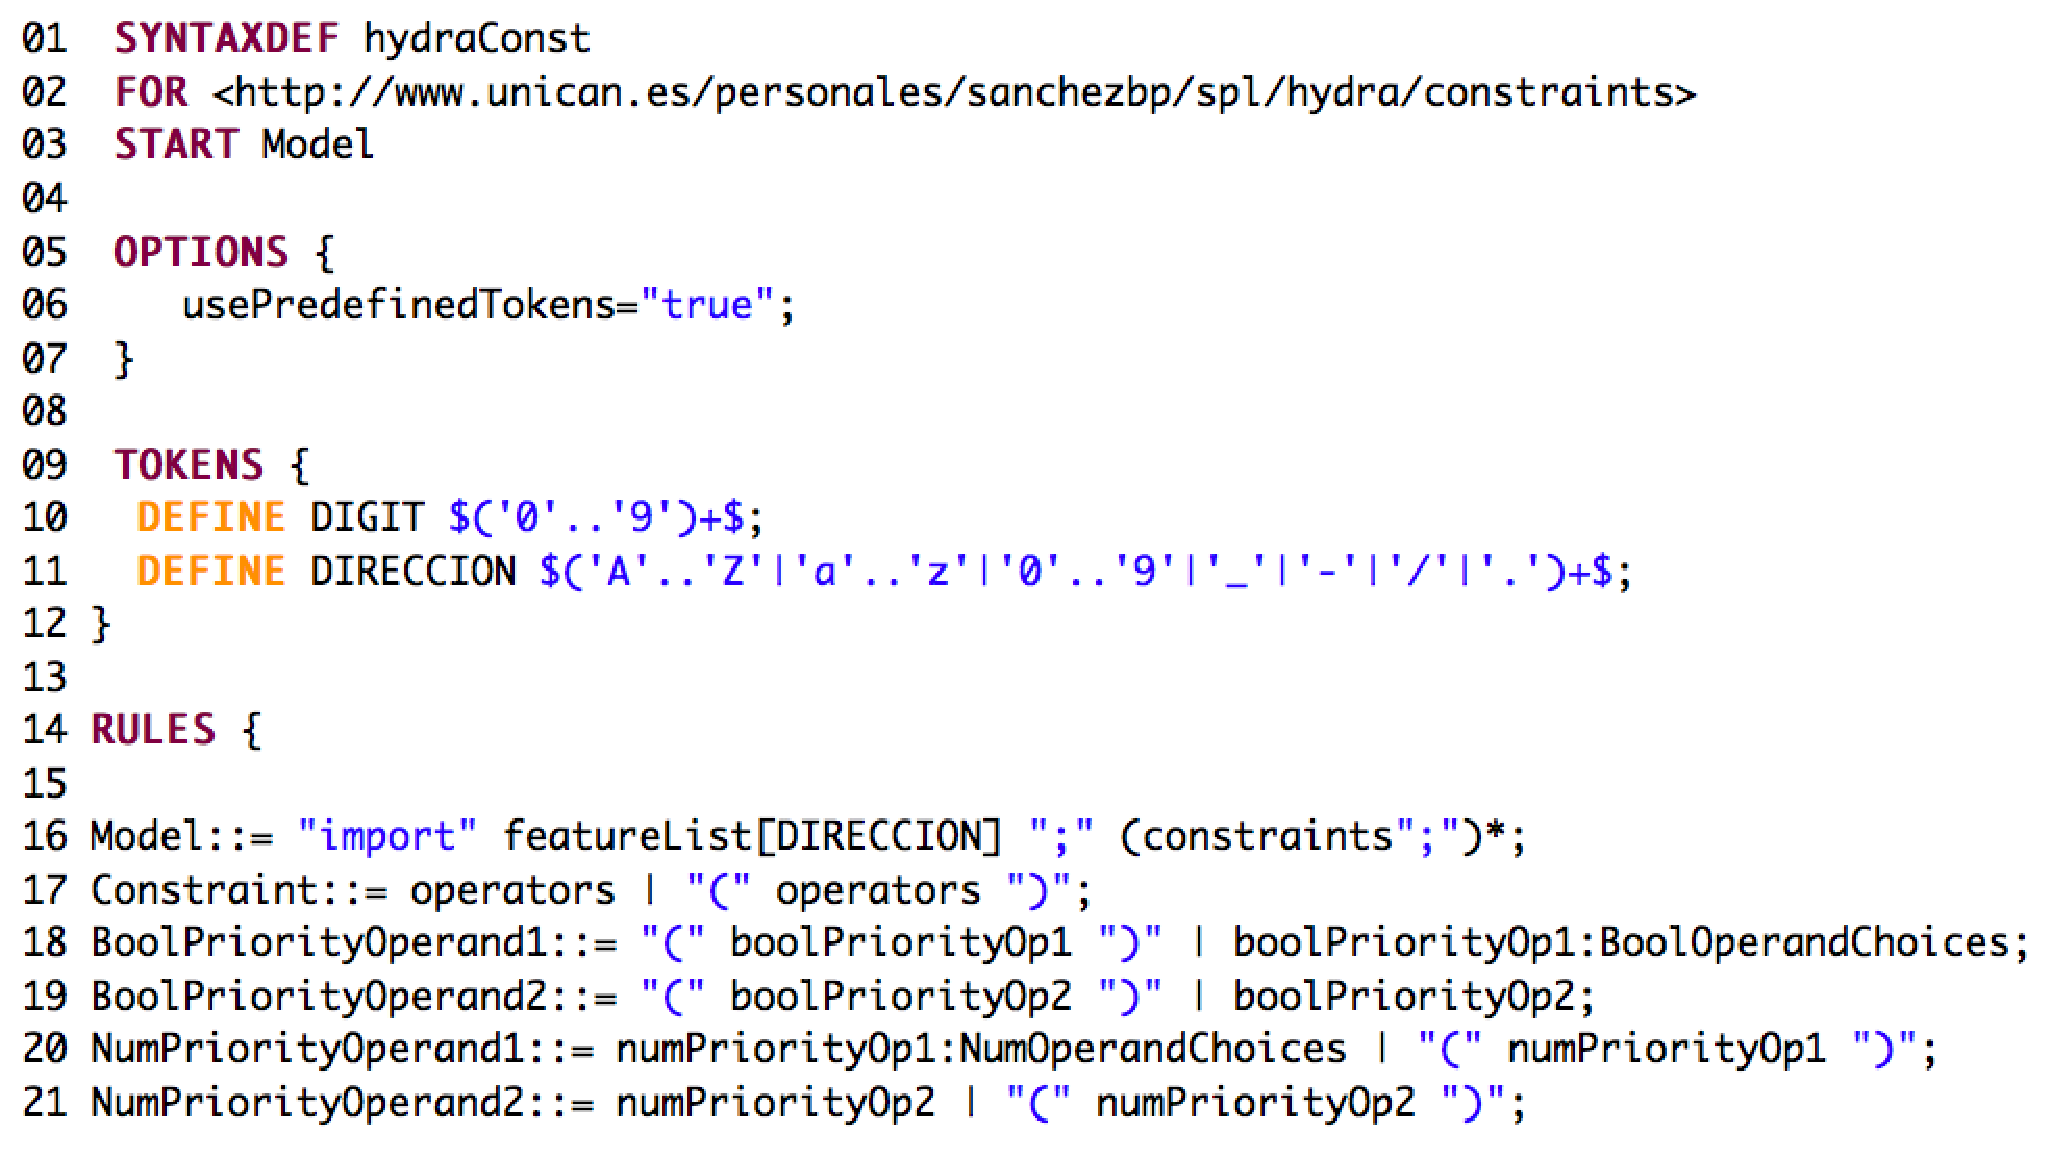
\includegraphics[scale=0.35]{gramatica/iniciogram.eps}
%\caption{Implementaci�n del inicio de la gram�tica con EMFText. Con la figura \ref{figopers} se completa la gram�tica}
%\label{figinitgram}
%\end{figure}
%
%\begin{figure}[t]
%    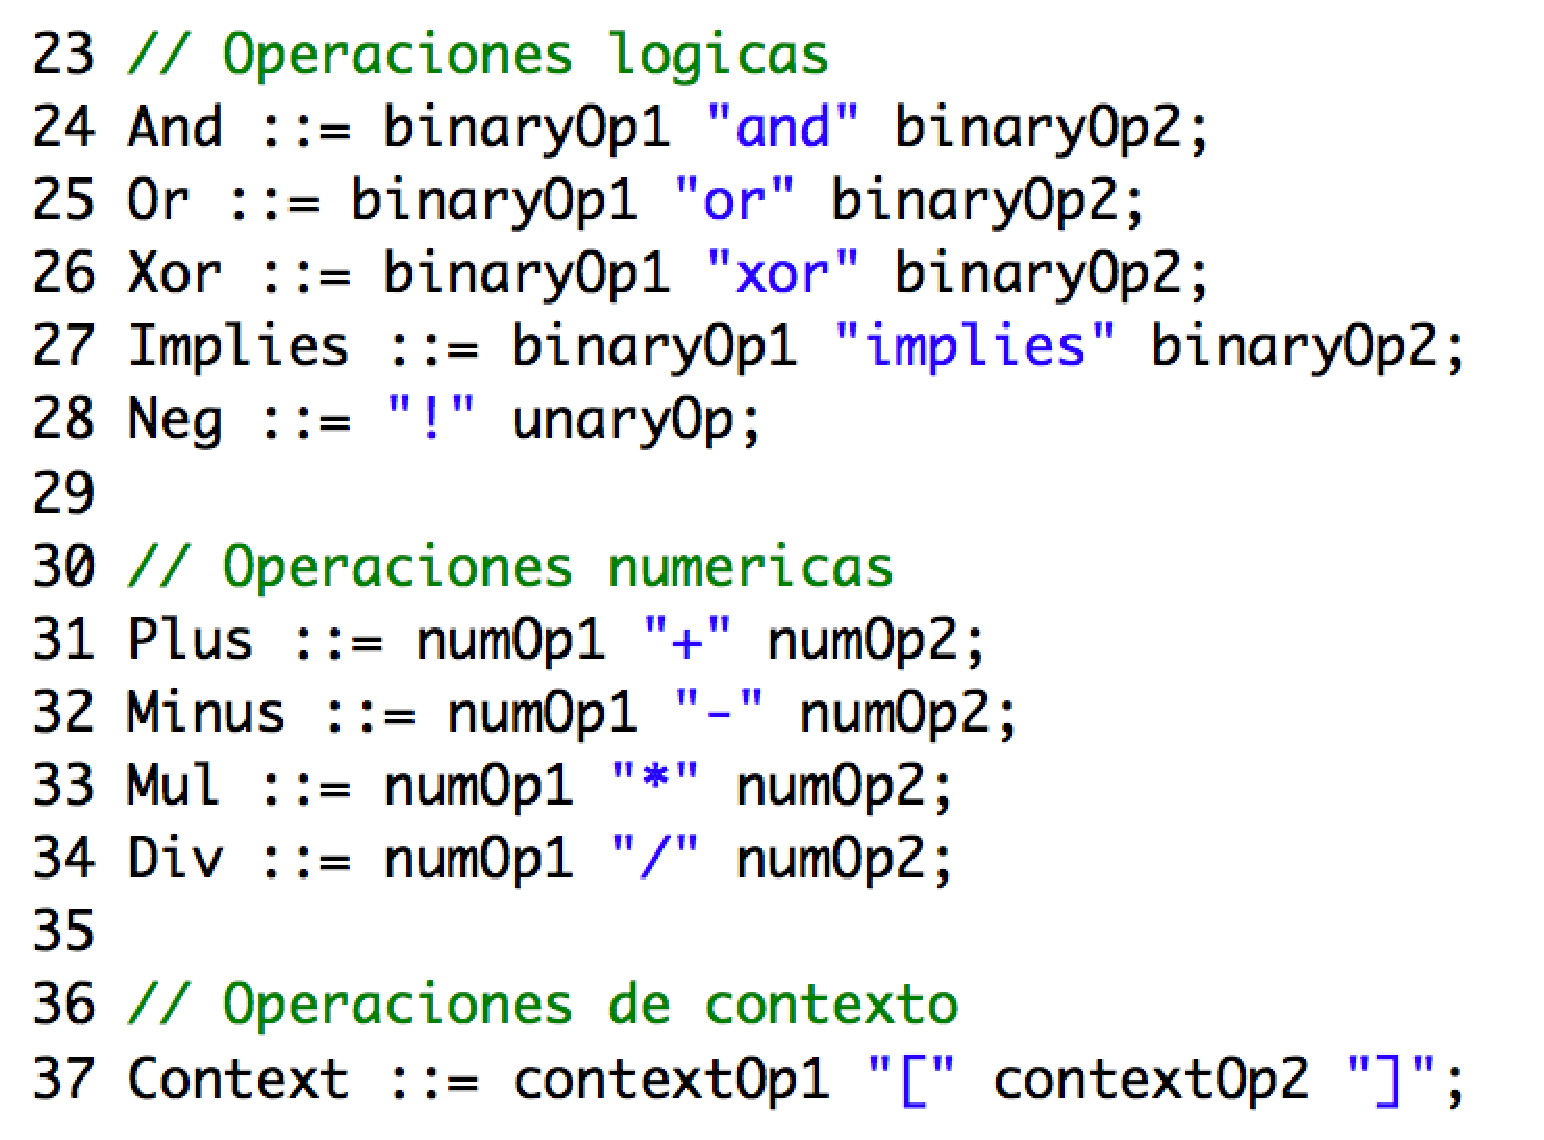
\includegraphics[scale=0.3]{gramatica/operaciones1.eps}
%    \caption{Implementaci�n de las operaciones de nuestro editor com EMFText}
%    \label{figopers}
%\end{figure}
%
%S� que cabe comentar con respecto a las operaciones las �ltimas l�neas, que muestran la asignaci�n de valor a las hojas de nuestros �rboles parseados. En esas l�neas estamos indicando que los atributos de las instancias de clase Number van a ser n�meros, y que los atributos de las instancias de las clases SimpleFeature y MultipleFeature van a ser palabras.
%
%La parte m�s complicada corresponde a la implementaci�n del inicio de la gram�tica y de las producciones que conducen a la misma. Pero antes de mostrar la figura con esta parte de la gram�tica conviene explicar el problema que llev� a realizar los cambios en el metamodelo mencionados en el cap�tulo anterior. Este problema surgi� a la hora de implementar las operaciones con prioridad, es decir, la inclusi�n de los par�ntesis.
%
%El inconveniente es que el tipo de gram�tica LL que implementa EMFText hac�a imposible tomar una decisi�n sobre hacia qu� elemento seguir parseando en caso de encontrarnos con un par�ntesis. La mejor soluci�n que se nos ocurri� para evitar este problema fue la adici�n de diversas clases y relaciones auxiliares en el metamodelo, cuya �nica funci�n es estructural y de apoyo a la gram�tica. Gracias a ellas y a una mejor definici�n de las producciones conseguimos evitar esos problemas de parsing y podemos llevar a cabo las operaciones de prioridad con par�ntesis.
%
%Las clases a�adidas para solventar esta situaci�n fueron las siguientes: BoolPriorityOperand1, BoolPriorityOperand2, NumPriorityOperand1, NumPriorityOperand2, BoolOperandChoices y NumOperandChoices. Las relaciones a�adidas fueron boolPriorityOp1, boolPriorityOp2, numPriorityOp1 y numPriorityOp2.
%
%Una situaci�n similar fue la que propici� que las operaciones Context, All y Any hayan sido dise�adas tal y como presenta el metamodelo, ya que que la particular sintaxis de estas (diferente a las dem�s que siguen el mismo esquema de op + char + op) tambi�n mostraba ciertos problemas de parsing. En este caso no fue necesario a�adir elementos auxiliares, sino simplemente recolocarlos para evitar estos problemas. Con esto ya se han hecho todos los cambios en el metamodelo, que alcanza en este punto su versi�n final tal como muestra la figura \ref{figmetameta}. Con respecto al metamodelo solamente quedan por comentar los m�todos que muestran algunas clases, que ser�n explicados en los pr�ximos cap�tulos ya que se usan en el proceso de validaci�n y sem�ntica.
%
%
%
%Una vez comentados estos detalles es momento de explicar el inicio de la gram�tica, que se muestra en la figura \ref{figinitgram}.
%
%En la primera l�nea y mediante la cla�sula SYNTAXDEF indicamos la extensi�n que queremos que tengan los ficheros escritos en nuestro lenguaje. En nuestro caso nos hemos decantado por la terminaci�n .hydraConst. En la segunda l�nea y mediante la cla�sula FOR se indica la URI del metamodelo. Una URI es un formato de direcci�n interno de Eclipse, que se usa para localizar otros ficheros en el workspace. En la tercera l�nea, delimitada por la cla�sula START, indicamos a la gram�tica que la clase inicial de nuestro metamodelo (y la que ser� la raiz en todos los �rboles parseados) es Model.
%
%El bloque OPTIONS permite activar algunas opciones de configuraci�n que incluye EMFText. En nuestro caso la �nica que tiene utilidad es usePredifinedTokens, que permite ahorrarnos la definici�n del token text. El bloque TOKENS sirve para definir los tokens de nuestra gram�tica. En nuestro caso usaremos 3: DIGIT para asignar al valor num�rico, TEXT para asignar a las caracter�sticas y DIRECCION para asignar la direcci�n f�sica del modelo de caracter�sticas.
%
%Por �ltimo, el bloque RULES permite crear las producciones. Como inicial, tal y como se especific� en los requisitos, exigimos un import y una direcci�n, que ser� almacenada en el atributo featureList de la clase Model. En la l�nea inicial tambi�n se indica, mediante una expresi�n regular, que el n�mero de restricciones a definir puede ser tan grande como se desee y que estas deben acabar con el car�cter '';'' .
%
%\begin{figure}[t]
%    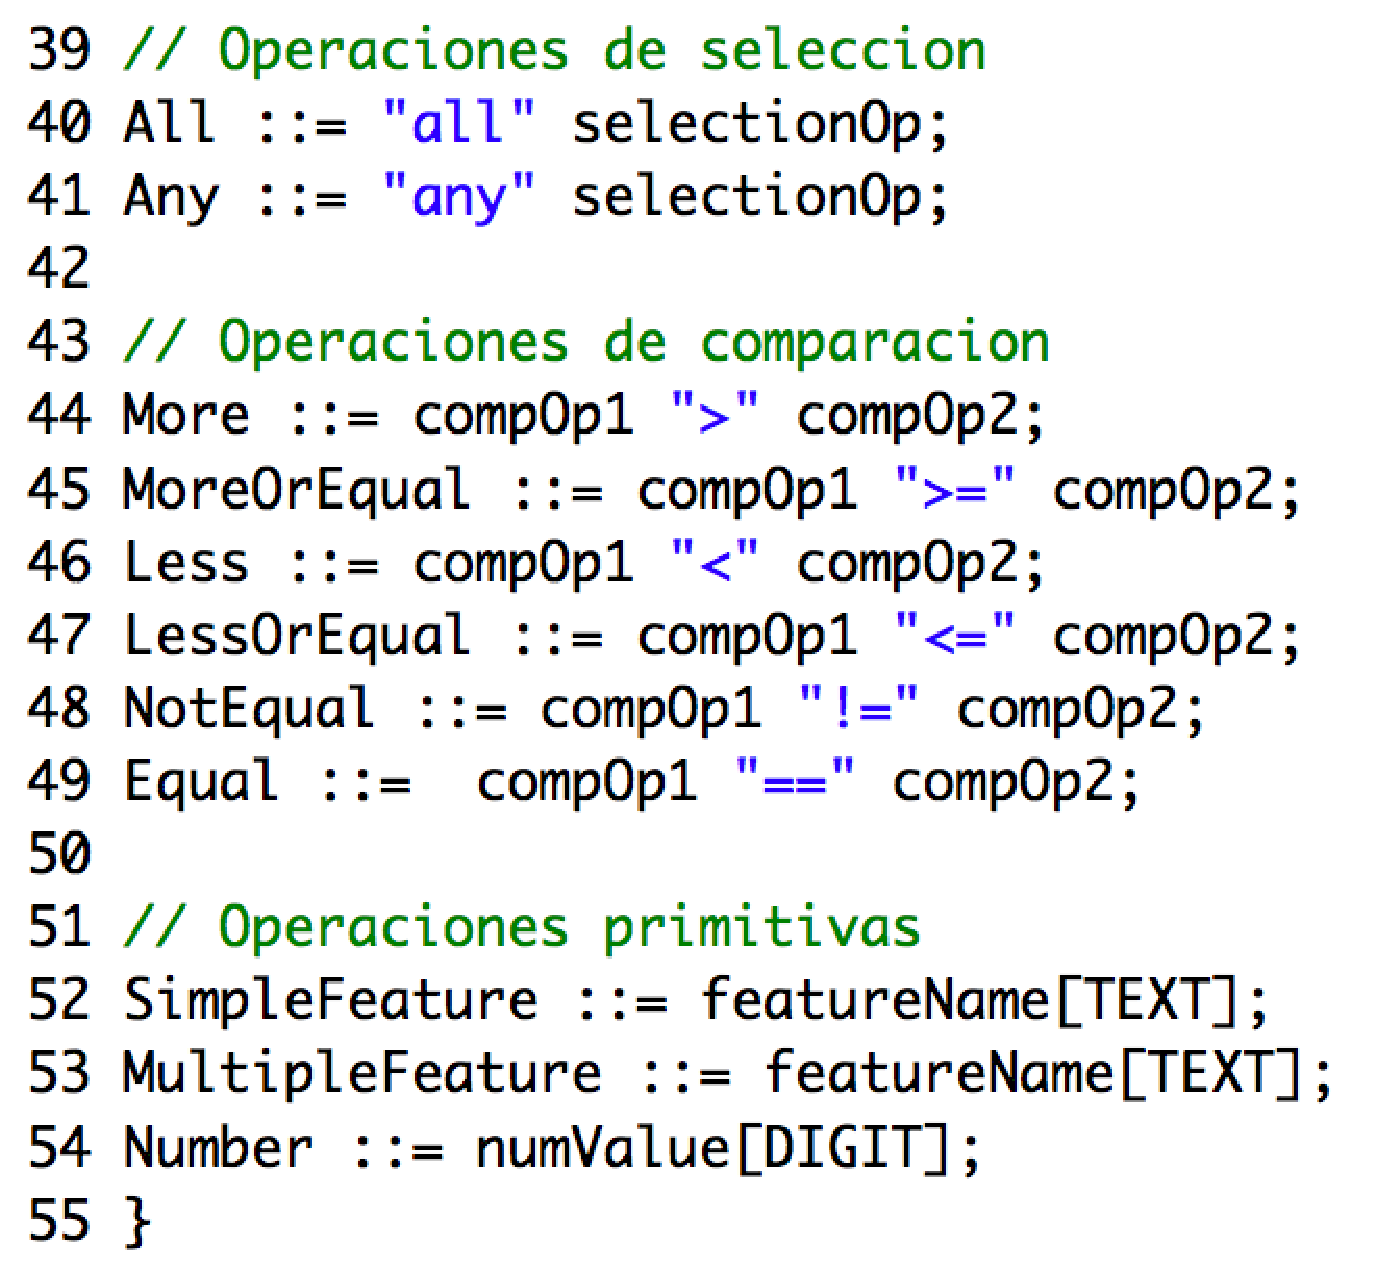
\includegraphics[scale=0.3]{gramatica/operaciones2.eps}
%    \caption{Implementaci�n de las operaciones de nuestro editor com EMFText}
%    \label{figopers}
%\end{figure}
%
%La l�nea de producci�n de Constraint diferencia entre operaciones con prioridad y sin ella. Sin el problema comentado de EMFText la gram�tica podr�a quedar as�, pero para solucionarlo nos vemos obligado a incluir las cuatro l�neas siguientes, cuya �nica funci�n es solventar esa situaci�n. El resto de la gram�tica continuar�a en la figura \ref{figopers} mostrada anteriormente, y ah� terminar�a.






\section{Pruebas}
\label{sec:gram:pruebas}
%%==================================================================%%
%% Author : Tejedo Gonz�lez, Daniel                                 %%
%%          S�nchez Barreiro, Pablo                                 %%
%% Version: 1.0, 25/11/2012                                         %%
%% Version: 1.0, 06/02/2013                                         %%
%%                                                                  %%
%% Memoria del Proyecto Fin de Carrera                              %%
%% Sintaxis abstracta,  pruebas                                     %%
%%==================================================================%%

Una vez creado nuestro metamodelo, deb�amos probar que dicho metamodelo era correcto. Es decir, que permit�a especificar todas las restricciones que dese�bamos crear, a la vez que, por construcci�n, imped�a la especificaci�n de restricciones que deb�an ser consideradas como sint�cticamente incorrectas.

Para ello realizamos una serie de pruebas consistentes en la creaci�n de varias instancias del metamodelo y observar el �rbol de sintaxis abstracta generado, comprobando si �ste se correspond�a con el esperado.

\begin{figure}[t]
    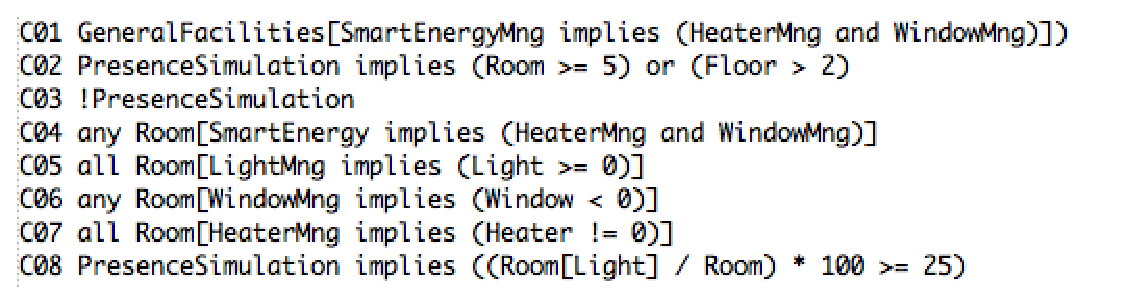
\includegraphics[scale=0.6]{metamodelo/instpruebas.eps}
    \caption{Conjunto de instrucciones que puso a prueba el funcionamiento del metamodelo}
    \label{figmetains}
\end{figure}

Las instrucciones que fueron puestas a prueba fueron las que se ven en la Figura~\ref{figmetains}. Este conjunto de instrucciones servir�n como pruebas tambi�n en momentos m�s avanzados del desarrollo. Dicho conjunto de pruebas fue dise�ado para recoger de la forma m�s exhaustiva posible todas las combinaciones de metaclases posibles.


%%=================================================================%%
%% NOTA(Pablo): A�ade una secci�n de sumario
%%=================================================================%%


\section{Sumario}
\label{sec:gram:sumario}
%%==================================================================%%
%% Author : Tejedo Gonz�lez, Daniel                                 %%
%%          S�nchez Barreiro, Pablo                                 %%
%% Version: 1.0, 25/11/2012                                         %%                   
%%                                                                  %%
%% Memoria del Proyecto Fin de Carrera                              %%
%% Sintaxis abstracta, sumario                          %%
%%==================================================================%%

Durante el presente cap�tulo se ha descrito el proceso de definici�n de la sintaxis abstracta de nuestro lenguaje. Este proceso abarca subtareas como la captura de requisitos del lenguaje, la creaci�n de un metamodelo que permita la creaci�n de sintaxis concretas apropiadas, la validaci�n de restricciones externas a ese metamodelo, y las pruebas que corroboren que todos los elementos creados funcionan correctamente. En el siguiente cap�tulo profundizaremos acerca del dise�o de la gram�tica para nuestro lenguaje, as� como de las herramientas utilizadas para implementar esa gram�tica.
